% Источник: Leontiev-2017.pdf; печатная страница: 13; страница файла: 13
\section*{Глава I. Основные понятия и уравнения теории фильтрации}
\subsection*{§ 3. Законы сохранения массы и импульса при фильтрации в пористой среде}
\label{q3:sec-3}
\setcounter{footnote}{0}
Введенные в предыдущих параграфах функции от пространственных координат и времени --- $p(x^i,t)$, $\rho(x^i,t)$, $m(x^i,t)$ и $\boldsymbol{u}(x^i,t)$\footnote{В некоторых задачах, конечно, может потребоваться введение и других параметров, например температуры жидкости, концентрации примесей в ней и т.д.} --- заранее, вообще говоря, неизвестны и должны находиться на основе уравнений, выражающих универсальные законы сохранения, а также специальных физических закономерностей для конкретных изучаемых явлений (например, уравнений состояния или законов электродинамики). В простейших случаях
% Источник: Leontiev-2017.pdf; печатная страница: 14; страница файла: 14
для получения замкнутой системы дифференциальных уравнений оказывается достаточным использовать только два закона сохранения --- уравнения баланса массы и импульса, к феноменологическому описанию которых мы переходим.

\topic{Закон сохранения массы}
Интегральная формулировка закона сохранения массы жидкости получается из утверждения о том, что изменение массы жидкости в произвольном объеме $V$ внутри пористой среды происходит за счет притока жидкости через границу объема $\Sigma$:
\[
\frac{d}{dt}\int_V\rho m\,dV=-\int_\Sigma\rho\boldsymbol{u}\cdot\boldsymbol{n}\,d\sigma.
\]
Здесь $\boldsymbol{n}$ --- вектор внешней нормали к поверхности $\Sigma$ (из-за такого выбора нормали интеграл в правой части стоит со знаком минус), а объем $V$ неподвижен относительно пористой среды. Если входящие в это уравнение функции являются достаточно гладкими, то в левой части можно занести производную под знак интеграла, а правую часть преобразовать с помощью теоремы Гаусса--Остроградского:
\[
\int_V\frac{\partial(\rho m)}{\partial t}\,dV=-\int_V\Div(\rho\boldsymbol{u})\,dV,
\]
откуда в силу произвольности объема $V$ получается дифференциальная запись закона сохранения массы --- \textit{уравнение неразрывности}:
\begin{equation}
\frac{\partial(\rho m)}{\partial t}+\Div(\rho\boldsymbol{u})=0.
\tag{3.1}\label{q3:eq-3-1}
\end{equation}
Если плотность жидкости постоянна, а пористая среда не деформируется (т.е. пористость зависит только от координат), то первое слагаемое обращается в ноль и уравнение неразрывности приобретает вид
\begin{equation}
\Div\boldsymbol{u}=0.
\tag{3.2}\label{q3:eq-3-2}
\end{equation}

\topic{Уравнение баланса импульса --- закон Дарси}
Исторически уравнение баланса импульса было экспериментально получено французским гидравликом Анр\'и Дарс\'и (H.Darcy, 1856) для случая медленного стационарного движения несжимаемой жидкости в неподвижной изотропной пористой
% Источник: Leontiev-2017.pdf; печатная страница: 15; страница файла: 15
среде. В современных обозначениях это соотношение, называемое \textit{законом Дарси}, для фильтрации в поле тяжести имеет вид
\begin{equation}
0=-\grad p+\rho\boldsymbol{g}-\frac{\mu}{k}\boldsymbol{u},
\tag{3.3}\label{q3:eq-3-3}
\end{equation}
где $\boldsymbol{g}$ --- ускорение свободного падения, $\mu$ --- коэффициент динамической вязкости жидкости, $k$ --- коэффициент, называемый проницаемостью пористой среды, который зависит от типа пористой среды. По структуре уравнение \eqref{q3:eq-3-3} похоже на уравнение Навье--Стокса для вязкой несжимаемой жидкости при $\mu=\mathrm{const}$:
\begin{equation}
\rho\frac{d\boldsymbol{v}}{dt}=-\grad p+\rho\boldsymbol{g}+\mu\triangle\boldsymbol{v}
\tag{3.4}\label{q3:eq-3-4}
\end{equation}
и это не удивительно: макроскопический закон движения при фильтрации в пористой среде (закон Дарси) может быть получен с помощью некоторой процедуры осреднения из уравнения движения, описывающего внутрипоровое движение жидкости на микроуровне, то есть уравнения Навье--Стокса (см. § 5). При медленных (ползущих) течениях внутри пористой среды, для которых и справедлив закон Дарси, инерционные силы много меньше вязких сил, поэтому сто\'ящим в левой части \eqref{q3:eq-3-4} ускорением можно пренебречь, что даст при осреднении ноль в левой части \eqref{q3:eq-3-3}. Наличие же последнего слагаемого в \eqref{q3:eq-3-4}, описывающего действие вязкости, приводит при переходе к макроскопическому описанию к появлению объемной силы вязкого сопротивления, действующей на жидкость со стороны пористого скелета. В рассматриваемом случае медленных течений\setcounter{footnote}{0}\footnote{Более точно --- при числах Рейнольдса $\Rey=\rho vd/\mu\ll1$.} в изотропной среде сила сопротивления направлена противоположно скорости фильтрации, а ее величина прямо пропорциональна вязкости и модулю скорости фильтрации.

При $\boldsymbol{g}=0$ закон Дарси приобретает вид
\begin{equation}
\boldsymbol{u}=-\frac{k}{\mu}\grad p;
\tag{3.5}\label{q3:eq-3-5}
\end{equation}
знак минус в правой части \eqref{q3:eq-3-5} имеет ясный физический смысл: в отсутствие массовых сил жидкость движется в пористой среде из областей с б\'ольшим давлением в области с меньшим давлением.

% Источник: Leontiev-2017.pdf; печатная страница: 16; страница файла: 16
Если жидкость в порах покоится ($\boldsymbol{u}=0$), то закон Дарси превращается, как и следует, в обычное уравнение равновесия жидкости
\[
0=-\grad p+\rho\boldsymbol{g}.
\]

\topic{Коэффициент проницаемости}
\setcounter{footnote}{0}
Коэффициент проницаемости $k$ зависит только от свойств пористой среды (но не от свойств жидкости), и определяется, в основном, геометрией порового пространства. Он имеет размерность площади, а его величина имеет порядок квадрата характерного размера пор $d$\footnote{Для зависимости проницаемости от геометрических характеристик пористой среды предлагалось большое число приближенных формул, которые основаны на различных простых моделях внутрипорового пространства [16, 18]. В качестве примера приведем часто используемую формулу Козени--Кармана (J.Kozeny, P.C.Carman): $k\sim d^2m^3/(1-m)^2$, где характерный размер пор $d$ вычисляется как отношение объема образца к площади поверхности пор. Для плотной упаковки одинаковых сферических частиц диаметром $D$ справедлива приближенная формула $k=2\cdot10^{-3}D^2$.}. Для примера укажем, что типичные значения проницаемости для песчаников имеют порядок $10^{-15}$--$10^{-12}$~м$^2$, для почв --- $10^{-13}$--$10^{-11}$~м$^2$\footnote{Для сигареты $k\sim10^{-9}$~м$^2$.}.

В практических приложениях часто в качестве единицы $k$ выбирают такую проницаемость, чтобы в отсутствие тяжести (см. \eqref{q3:eq-3-5}) при градиенте давления\footnote{Килограмм-сила --- единица силы в технической системе единиц, приближенно равная весу эталона килограмма у поверхности земли: $1$~кгс $=9{,}80665$~Н $\approx9{,}81$~Н.} $1$~кгс/см$^3\approx1$~атм/см жидкость с вязкостью $0{,}01$~г/(см$\cdot$с) (вязкость воды при $20^\circ$C) имела скорость фильтрации $1$~см/с. Эта единица проницаемости называется \textit{дарси} (обозначение «Д»); $1$~Д $\approx1{,}02\cdot10^{-12}$~м$^2\approx1$~мкм$^2$.

Для неоднородных пористых сред коэффициент проницаемости является функцией пространственных координат и может меняться с течением времени (например, при деформациях пористого скелета или за счет его засорения или растворения).

\topic{Коэффициент фильтрации}
В гидротехнической практике закон Дарси обычно используется в виде уравнения, разрешенного относительно скорости фильтрации, причем вместо давления используется
% Источник: Leontiev-2017.pdf; печатная страница: 17; страница файла: 17
\textit{пьезометрический напор} (или просто \textit{напор})\setcounter{footnote}{0}\footnote{Напор имеет размерность длины и с точностью до постоянного слагаемого равен вертикальной координате свободной поверхности жидкости в измерительной скважине, пробуренной в пористый пласт, чем и объясняется удобство его использования.}
\[
H=H(x,y,z,t)=\frac{p}{\rho g}+z,
\]
где $z$ --- вертикальная координата рассматриваемой точки (ось $Oz$ направлена вверх, противоположно $\boldsymbol{g}$). Выразив скорость фильтрации из \eqref{q3:eq-3-3}, получим
\begin{equation}
\boldsymbol{u}=-C\grad H,\qquad C=\frac{k\rho g}{\mu},
\tag{3.6}\label{q3:eq-3-6}
\end{equation}
где $C$ --- \textit{коэффициент фильтрации}, зависящий, очевидно, как от свойств пористой среды, так и от свойств жидкости\footnote{В англоязычной литературе величину $C$ обычно называют «гидравлической проводимостью» (\textit{hydraulic conductivity}).}. Типичные значения $C$ при фильтрации воды в песке имеют порядок $10^{-5}$--$10^{-2}$~м/с, в почве --- $10^{-6}$--$10^{-4}$~м/с, в глине --- $10^{-7}$--$10^{-6}$~м/с.

\topic{Закон Дарси для анизотропных сред}
При фильтрации в анизотропных пористых средах (например, в осадочных слоистых пластах или в средах с трещинами, направленными в выделенном направлении) линейная зависимость скорости фильтрации и градиента давления сохраняется (для медленных течений), однако эти векторы в случае общего положения уже не будут параллельны. Проницаемость таких сред будет характеризоваться не одним числом (коэффициентом проницаемости $k$), а симметричным положительно-определенным \textit{тензором проницаемости} $k_{ij}$, входящим в закон Дарси
\[
u_i=-\frac{k_{ij}}{\mu}(\nabla^jp-\rho g^j).
\]
Например, в слоистой среде, у которой направление, перпендикулярное плоскости напластования, задается единичным вектором $\boldsymbol{n}$, тензор проницаемости в декартовой системе координат имеет вид
\[
k_{ij}=(k_\perp-k_\parallel)n_in_j+k_\parallel\delta_{ij},
\]
где $k_\perp$ и $k_\parallel$ суть проницаемости при фильтрации соответственно поперек и вдоль напластования.


% Источник: Leontiev-2017.pdf; печатная страница: 24; страница файла: 24
\subsection*{§ 5. Вывод дифференциальных уравнений фильтрации с помощью осреднения микроскопических уравнений}
\label{q3:sec-5}
Как уже говорилось, уравнения теории фильтрации могут быть получены осреднением уравнений, описывающих внутрипоровое движение жидкости на микроуровне. Эта процедура проводится следующим образом.

\topic{Осреднение параметров жидкости в пористой среде}
\setcounter{footnote}{1}
Предположим, что мы хотим осреднить некоторую физическую величину $A(x^k,t)$, определенную в жидкости (скажем, давление). Поскольку в тех областях, где жидкость отсутствует (в пористом скелете), величина $A$, вообще говоря, не определена, доопределим ее в этих областях нулевым значением, и вычислим в некоторый момент времени среднее значение $A$ по сфере $V$ некоторого фиксированного радиуса с центром в точке $(x_0;y_0;z_0)$ (рис.~\ref{q3:fig-7}):
\[
\langle A\rangle=\frac{1}{|V|}\int_V A\,dV,
\]
где $|V|$ --- объем сферы\footnote{Вместо сферы можно взять объем какой-либо другой формы, например эллипсоид или параллелепипед с заданной фиксированной ориентацией относительно осей координат.}. Так полученное среднее значение $\langle A\rangle$ является непрерывной и почти всюду дифференцируемой функцией
% Источник: Leontiev-2017.pdf; печатная страница: 25; страница файла: 25
координат центра объема и времени:
\[
\langle A\rangle=\langle A\rangle(x_0,y_0,z_0,t),
\]
причем $\langle A\rangle$ будет уже определена \textit{везде} в рассматриваемой области, даже если точка $(x_0;y_0;z_0)$ попадает внутрь пористого скелета\setcounter{footnote}{0}\footnote{Обратим внимание, что исходная величина $A$ зависит не от $x_0^i$, а от $x^i$.}. В дальнейшем для упрощения обозначений индекс «0» при записи производных будет опускаться.

\topic{Свойства операции осреднения}
Операция осреднения, очевидно, линейна:
\[
\langle cA\rangle=c\langle A\rangle,\quad \langle A+B\rangle=\langle A\rangle+\langle B\rangle,\quad c=\mathrm{const},
\]
\setcounter{figure}{6}
\begin{figure}[H]
\centering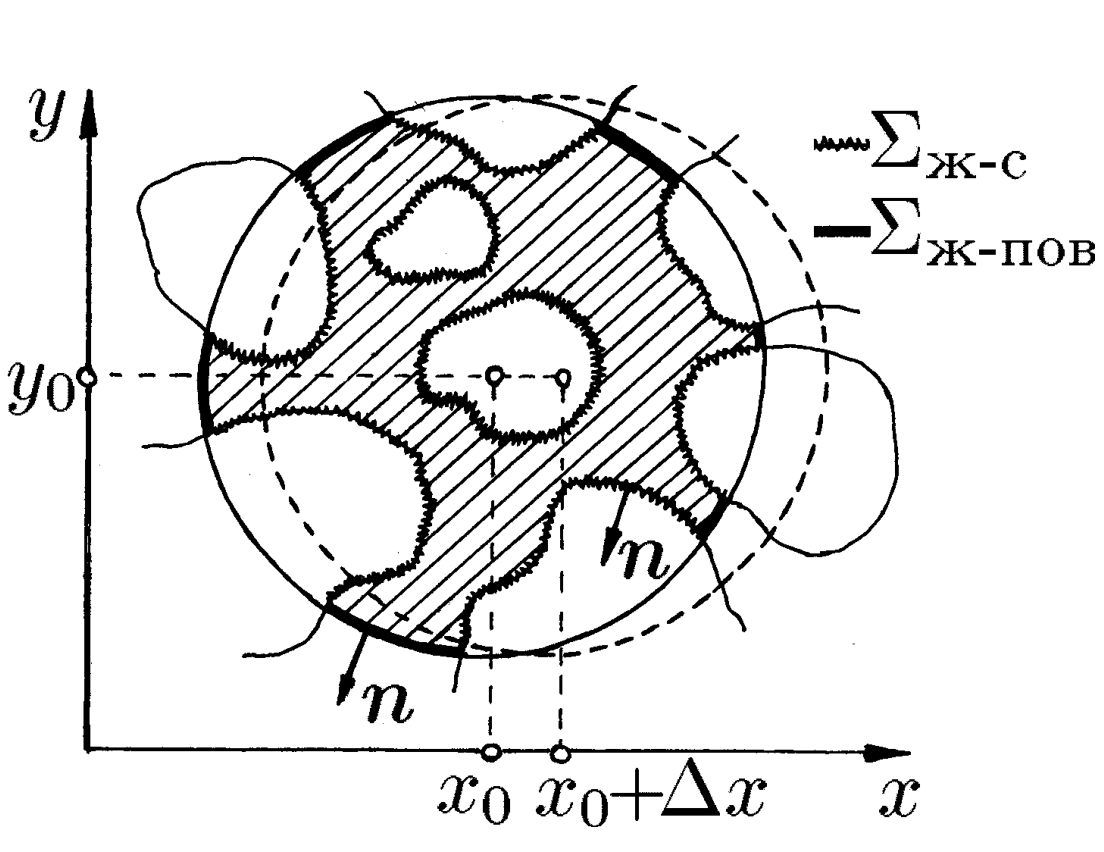
\includegraphics[width=.53\linewidth]{figures/figure-7.png}
\caption{}\label{q3:fig-7}
\end{figure}
а среднее значение единичной функции (доопределенной нулем внутри пористого скелета) равно средней пористости той части среды, которая попадает внутрь объема $V$: $\langle1\rangle=m$.

В случае \textit{недеформируемого неподвижного} пористого скелета, которым мы для простоты ограничимся, при вычислении среднего от производных справедливы равенства
\begin{equation}
\left\langle\frac{\partial A}{\partial t}\right\rangle=\frac{\partial\langle A\rangle}{\partial t},\qquad
\left\langle\frac{\partial A}{\partial x^i}\right\rangle=\frac{\partial\langle A\rangle}{\partial x^i}+\frac{1}{|V|}\int_{\Sigma_{\text{ж-с}}}An_i\,d\sigma,
\tag{5.1}\label{q3:eq-5-1}
\end{equation}
где $\Sigma_{\text{ж-с}}$ --- граница жидкости и скелета, попадающая внутрь $V$, $\boldsymbol{n}=(n_x;n_y;n_z)$ --- вектор внешней нормали к заштрихованному на рис.~\ref{q3:fig-7} объему $V_{\text{ж}}$ жидкости, находящейся внутри сферы.

Доказательство первой формулы очевидно, для доказательства второй формулы нужно заметить, что при малом смещении объема $V$ вдоль, например, оси $x$ на расстояние $\Delta x$ (рис.~\ref{q3:fig-7}) среднее значение $A$ меняется в основном за счет того, что к объему добавляется или из него
% Источник: Leontiev-2017.pdf; печатная страница: 26; страница файла: 26
исключается тонкий слой жидкости, расположенный вдоль $\Sigma_{\text{ж-пов}}$ --- границы жидкости и поверхности сферы:
\[
\begin{aligned}
\frac{\partial\langle A\rangle}{\partial x}
&=\lim_{\Delta x\to0}\frac{\langle A\rangle(x_0+\Delta x,y_0,z_0)-\langle A\rangle(x_0,y_0,z_0)}{\Delta x}\\
&=\frac{1}{|V|}\int_{\Sigma_{\text{ж-пов}}}An_x\,d\sigma.
\end{aligned}
\]
Остается представить полученный интеграл по одной части границы объема $V_{\text{ж}}$ как разность интегралов по всей границе и по $\Sigma_{\text{ж-с}}$ --- по оставшейся части, и к первому интегралу применить теорему Гаусса--Остроградского:
\[
\begin{aligned}
\frac{\partial\langle A\rangle}{\partial x}
&=\frac{1}{|V|}\int_{V_{\text{ж}}}\frac{\partial A}{\partial x}\,dV-\frac{1}{|V|}\int_{\Sigma_{\text{ж-с}}}An_x\,d\sigma\\
&=\frac{1}{|V|}\int_V\frac{\partial A}{\partial x}\,dV-\frac{1}{|V|}\int_{\Sigma_{\text{ж-с}}}An_x\,d\sigma.
\end{aligned}
\]
Теперь с помощью \eqref{q3:eq-5-1} несложно получить осредненные уравнения фильтрации. Проделаем это для случая однородной \textit{несжимаемой} ньютоновской жидкости.

\topic{Осреднение микроскопического уравнения неразрывности}
Осреднение уравнения неразрывности $\Div\boldsymbol{v}=0$ производится очень просто:
\[
\langle\nabla_iv^i\rangle=\nabla_i\langle v^i\rangle+\frac{1}{|V|}\int_{\Sigma_{\text{ж-с}}}v^in_i\,d\sigma=0,
\]
откуда с учетом условия прилипания получаем выражение закона сохранения массы в терминах средних параметров:
\begin{equation}
\nabla_i\langle v^i\rangle\equiv\Div\langle\boldsymbol{v}\rangle=0.
\tag{5.2}\label{q3:eq-5-2}
\end{equation}
Величина, стоящая под знаком дивергенции, есть не что иное, как скорость фильтрации:
\[
\langle\boldsymbol{v}\rangle=\boldsymbol{u},
\]
так что \eqref{q3:eq-5-2} совпадает с \eqref{q3:eq-3-2}.

\topic{Осреднение микроскопического уравнения движения}
Для осреднения удобно взять уравнение движения в дивергентном виде
\[
\rho\left(\frac{\partial v^i}{\partial t}+\nabla_k(v^kv^i)\right)=\nabla_kp^{ik}+\rho F^i,
\]
в котором $p^{ik}$ --- компоненты тензора напряжений, $F^i$ --- компоненты вектора массовой плотности внешних объемных сил. Применяя \eqref{q3:eq-5-1} и учитывая условие прилипания, получим
\[
\rho\left(\frac{\partial\langle v^i\rangle}{\partial t}+\nabla_k\langle v^kv^i\rangle\right)=\nabla_k\langle p^{ik}\rangle+F^i_{\text{с-ж}}+\rho\langle F^i\rangle,
\]
\[
F^i_{\text{с-ж}}=\frac{1}{|V|}\int_{\Sigma_{\text{ж-с}}}p^{ik}n_k\,d\sigma,
\]
% Источник: Leontiev-2017.pdf; печатная страница: 27; страница файла: 27
где сила $\boldsymbol{F}_{\text{с-ж}}$, вид которой будет обсуждаться чуть позже, представляет собой \textit{полную} силу (в расчете на единицу объема), действующую со стороны скелета на жидкость внутри объема $V$, т.е. включает в себя как результат действия вязких касательных напряжений, так и результат суммирования нормальных напряжений на границе жидкости и скелета. Первое слагаемое в правой части, снова с учетом условия прилипания, принимает вид
\[
\begin{aligned}
\nabla_k\langle p^{ik}\rangle
&=\nabla_k\left\langle-pg^{ik}+\mu(\nabla^iv^k+\nabla^kv^i)\right\rangle=\\
&=-\nabla^i\langle p\rangle+\cancel{\mu\nabla_k\nabla^i\langle v^k\rangle}+\mu\nabla_k\nabla^k\langle v^i\rangle,
\end{aligned}
\]
где зачеркнутый член пропадает вследствие \eqref{q3:eq-5-2}, что в результате дает
\begin{equation}
\begin{aligned}
\rho\left(\frac{\partial\langle v^i\rangle}{\partial t}+\nabla_k\langle v^kv^i\rangle\right)
&=-\nabla^i\langle p\rangle+\mu\triangle\langle v^i\rangle\\
&\quad+\rho\langle F^i\rangle+F^i_{\text{с-ж}}.
\end{aligned}
\tag{5.3}\label{q3:eq-5-3}
\end{equation}
Уравнение \eqref{q3:eq-5-3} является точным, и дальнейшее его упрощение связанно с дополнительными гипотезами и оценкой входящих в него членов.
% Сохранено написание оригинала «связанно».

\topic{Упрощение уравнения движения при малых скоростях}
При малых скоростях течения порядок силы $F_{\text{с-ж}}$ (в однородной среде) в можно оценить, моделируя пористую среду системой капилляров с характерным поперечным размером $d$ или решеткой из частиц с характерным диаметром $d$, что дает в обоих случаях оценку
% Сохранена опечатка оригинала «(в однородной среде) в можно».
\[
F_{\text{с-ж}}\sim\frac{\mu u}{d^2}.
\]
Оценки порядков других членов \eqref{q3:eq-5-3}, содержащих скорость, дают\setcounter{footnote}{0}\footnote{Мы пользуемся тем, что производная $\frac{\partial A}{\partial x}$ имеет порядок $\delta A/L$, где $\delta A$ и $L$ --- характерные масштабы диапазонов изменения соответственно величины $A$ и независимой переменной $x$.}
\[
\frac{\rho\dfrac{\partial\langle v^i\rangle}{\partial t}}{F_{\text{с-ж}}}\sim\frac{\rho d^2}{\mu\tau},\qquad
\frac{\rho\nabla_k\langle v^kv^i\rangle}{F_{\text{с-ж}}}\sim\frac{\rho ud}{\mu}\cdot\frac{d}{L}=\Rey\cdot\frac{d}{L}\ll1,
\]
\[
\frac{\mu\triangle\langle v^i\rangle}{F_{\text{с-ж}}}\sim\left(\frac{d}{L}\right)^2\ll1,
\]
% Источник: Leontiev-2017.pdf; печатная страница: 28; страница файла: 28
где $\tau$ --- характерное время процесса. Подставив в первую оценку типичные значения определяющих параметров ($\rho\sim1$~г/см$^3$, $d\sim10^{-3}$~см, $\mu\sim10^{-2}$~г/(см$\cdot$с)), получим, что отношение нестационарного члена к $F_{\text{с-ж}}$ имеет порядок $\tau_*/\tau$, $\tau_*=10^{-4}$~с, т.е. нестационарный член нужно учитывать только в высокочастотных процессах. В результате, с учетом равенств
\[
\langle p\rangle=mp,\quad\langle\boldsymbol{F}\rangle=m\boldsymbol{F},
\]
где в правых частях (без символов осреднения) стоят средние значения $p$ и $\boldsymbol{F}$ \textit{по жидкой фазе} внутри объема $V$\setcounter{footnote}{0}\footnote{Обратим внимание, что среднее значение давления \textit{по жидкой фазе} --- это как раз та величина, которую покажет манометр, помещенный в жидкость внутри пор.}, получается уравнение движения для медленных течений
\[
0=-\grad(mp)+m\rho\boldsymbol{F}+\boldsymbol{F}_{\text{с-ж}}.
\]
В общем случае неоднородной пористой среды (при переменной пористости $m(x^i)$) сила $\boldsymbol{F}_{\text{с-ж}}$ не сводится только к силе трения, связанной с действием вязкости. Например, в отсутствие течения и массовых сил ($\boldsymbol{u}=0$, $\boldsymbol{F}=0$) сила межфазного взаимодействия $\boldsymbol{F}_{\text{с-ж}}=p\grad m\neq0$\footnote{Происхождение этой силы несложно понять в частном случае, рассматривая воздействие на жидкость со стороны стенок сужающегося капилляра.}.

Удобно выделить в явном виде \textit{силу сопротивления} (в расчете \textit{на единицу объема жидкости}), связанную --- прямо или косвенно --- с действием вязких сил и обращающуюся в ноль при $\boldsymbol{u}=0$, и переписать уравнение движения в виде
\begin{equation}
\begin{gathered}
0=-\grad p+\rho\boldsymbol{F}+\boldsymbol{F}_{\text{сопр}},\\
\boldsymbol{F}_{\text{сопр}}=\frac{1}{m}(\boldsymbol{F}_{\text{с-ж}}-p\grad m).
\end{gathered}
\tag{5.4}\label{q3:eq-5-4}
\end{equation}
Отметим, что если жидкость внутри пор покоится, то $\boldsymbol{F}_{\text{сопр}}=0$ даже при отличных от нуля массовых силах, хотя, скажем, при наличии тяжести \textit{на отдельное зерно} пористой среды со стороны жидкости будет действовать ненулевая выталкивающая сила Архимеда. Это связано с тем, что сила $\boldsymbol{F}_{\text{с-ж}}$ вычисляется для объема $V$, размеры которого $l$, в соответствии с (1.1), много больше размера пор $d$, так что сила со стороны жидкости на зёрна, \textit{целиком} находящиеся внутри $V$ (рис.~\ref{q3:fig-7}),
% Источник: Leontiev-2017.pdf; печатная страница: 29; страница файла: 29
уравновешивается силой, которая действует на зерна, \textit{пересекающие границу объема} $V$\setcounter{footnote}{0}\footnote{Разумеется, это может быть неверно, если размеры объема $V$ соизмеримы с размером зерен $d$.}.

В случае постоянной пористости закон \eqref{q3:eq-5-4} должен совпадать с законом Дарси, поэтому сила сопротивления
\[
\boldsymbol{F}_{\text{сопр}}=\frac{1}{m}\boldsymbol{F}_{\text{с-ж}}=-\frac{\mu}{k}\boldsymbol{u}.
\]
Подчеркнем, что даже в случае постоянной пористости и при малых скоростях течения $\boldsymbol{F}_{\text{сопр}}$ является, в общем случае, суммой не только касательных, но и нормальных напряжений\footnote{Сравните это с теми известными фактами [8], что при ползущем течении вязкой жидкости вокруг сферы одна треть стоксовской силы сопротивления складывается из воздействия нормальных напряжений, а при обтекании тонкой пластинки, расположенной поперек потока, вообще вся сила сопротивления обязана своим происхождением нормальным напряжениям.}.

\topic{Осреднение микроскопического уравнения энергии}
При выводе уравнения баланса энергии кроме операции $\langle\ \rangle$ осреднения величин, относящихся к жидкости, нам потребуется операция $\langle\ \rangle_{\text{с}}$ осреднения величин, определенных внутри скелета. Она определяется таким же образом:
\[
\langle A\rangle_{\text{с}}=\frac{1}{|V|}\int_V A\,dV
\]
с той лишь разницей, что теперь величина $A$ определена внутри скелета и доопределяется нулем внутри жидкости. Для осреднения по скелету выполняются равенства, аналогичные \eqref{q3:eq-5-1}:
\begin{equation}
\begin{aligned}
\left\langle\frac{\partial A}{\partial t}\right\rangle_{\text{с}}&=\frac{\partial\langle A\rangle_{\text{с}}}{\partial t},\\
\left\langle\frac{\partial A}{\partial x^i}\right\rangle_{\text{с}}&=\frac{\partial\langle A\rangle_{\text{с}}}{\partial x^i}-\frac{1}{|V|}\int_{\Sigma_{\text{ж-с}}}An_i\,d\sigma;
\end{aligned}
\tag{5.5}\label{q3:eq-5-5}
\end{equation}
знак минус перед интегралом связан с выбором направления нормали (теперь она направлена внутрь среды, по которой производится осреднение).

Осреднение уравнения энергии для жидкости
\[
\begin{aligned}
\frac{\partial}{\partial t}\left(\rho\left(U+\frac{v^2}{2}\right)\right)
&+\nabla_k\left(\rho v^k\left(U+\frac{v^2}{2}\right)\right)=\\
&=\rho F_kv^k+\nabla_k(p^{ik}v_i)-\nabla_kq^k+\rho Q
\end{aligned}
\]
% Источник: Leontiev-2017.pdf; печатная страница: 30; страница файла: 30
и уравнения энергии для скелета
\[
\frac{\partial}{\partial t}(\rho_{\text{с}}U_{\text{с}})=-\nabla_kq_{\text{с}}^k+\rho_{\text{с}}Q_{\text{с}},
\]
где $U$ и $Q$ --- массовые плотности соответственно внутренней энергии и объемного притока энергии, $\boldsymbol{q}$ --- вектор потока тепла, а индекс «с» обозначает величины, относящиеся к скелету, дает, с учетом условия прилипания, уравнения
\[
\begin{aligned}
\frac{\partial}{\partial t}\left\langle\rho\left(U+\frac{v^2}{2}\right)\right\rangle
&+\nabla_k\left\langle\rho v^k\left(U+\frac{v^2}{2}\right)\right\rangle=\\
&=\langle\rho F_kv^k\rangle+\nabla_k\langle p^{ik}v_i\rangle-\nabla_k\langle q^k\rangle\\
&\quad-\frac{1}{|V|}\int_{\Sigma_{\text{ж-с}}}q^kn_k\,d\sigma+\rho\langle Q\rangle,
\end{aligned}
\]
\[
\frac{\partial}{\partial t}\langle\rho_{\text{с}}U_{\text{с}}\rangle_{\text{с}}
=-\nabla_k\langle q_{\text{с}}^k\rangle_{\text{с}}+\frac{1}{|V|}\int_{\Sigma_{\text{ж-с}}}q_{\text{с}}^kn_k\,d\sigma+\rho_{\text{с}}\langle Q_{\text{с}}\rangle_{\text{с}},
\]
при сложении которых интегральные члены сокращаются (в силу условия $(\boldsymbol{q}-\boldsymbol{q}_{\text{с}})\cdot\boldsymbol{n}=0$ сохранения потока энергии на контактном разрыве --- границе жидкости и скелета), в результате чего получается требуемое уравнение энергии
\begin{equation}
\begin{aligned}
\frac{\partial}{\partial t}\left\{\left\langle\rho\left(U+\frac{v^2}{2}\right)\right\rangle+\langle\rho_{\text{с}}U_{\text{с}}\rangle_{\text{с}}\right\}
&+\nabla_k\left\langle\rho v^k\left(U+\frac{v^2}{2}\right)\right\rangle=\\
&=\langle\rho F_kv^k\rangle+\nabla_k\langle p^{ik}v_i\rangle\\
&\quad-\nabla_k\bigl(\langle q^k\rangle+\langle q_{\text{с}}^k\rangle_{\text{с}}\bigr)\\
&\quad+\rho\langle Q\rangle+\rho_{\text{с}}\langle Q_{\text{с}}\rangle_{\text{с}}.
\end{aligned}
\tag{5.6}\label{q3:eq-5-6}
\end{equation}

\topic{Упрощение уравнения энергии}
Этому уравнению можно придать более простой вид, если сделать следующие дополнительные предположения, выполняющиеся во многих практических приложениях.
\begin{enumerate}\sloppy
\item[а)] Кинетической энергией жидкости при движении внутри пор можно пренебречь по сравнению со внутренней энергией (в промысловых условиях $U\sim10^4$--$10^6$~м$^2$/с$^2$ $\gg v^2/2$).
\item[б)] Объемные притоки энергии отсутствуют: $Q=Q_{\text{с}}=0$.
\item[в)] Температуры жидкости и скелета можно считать одинаковыми, так как характерное время выравнивания их температур $t_*\sim\rho cd^2/\varkappa$, где $c$ и $\varkappa$ --- коэффициенты теплоемкости и теплопроводности, мало по сравнению с характерным временем фильтрационных процессов (величина $t_*$ для песка с $d\sim10^{-2}$~см порядка $10^{-1}$~с).
% Источник: Leontiev-2017.pdf; печатная страница: 31; страница файла: 31
\item[г)] Давление и температура являются медленно меняющимися функциями пространственных координат, в то время как скорость жидкости внутри пор является быстро меняющейся функцией. Это позволяет приближенно выполнять осреднение произведений:
\[
\langle pv^k\rangle\approx p\langle v^k\rangle=pu^k,\quad
\langle\rho Uv^k\rangle\approx\rho U\langle v^k\rangle=\rho Uu^k
\]
(в правых частях равенств стоят средние значения $p$, $U$ \textit{по жидкой фазе}).
\item[д)] В слагаемом, содержащем компоненты тензора напряжений, при осреднении можно пренебречь тензором вязких напряжений $\tau^{ij}$:
\[
\begin{aligned}
\nabla_k\langle p^{ik}v_i\rangle
&=-\nabla_k\langle pv^k\rangle+\nabla_k\langle\tau^{ik}v_i\rangle\\
&\approx-\nabla_k\bigl(p\langle v^k\rangle\bigr)=-\Div(p\boldsymbol{u}).
\end{aligned}
\]
В самом деле, $\tau^{ij}\sim\mu u/d$, а порядок изменения давления $\delta p$ (в масштабах задачи $L$) оценивается с помощью закона Дарси: $\delta p/L\sim\mu u/d^2$, откуда $\tau^{ij}/\delta p\sim d/L\ll1$. С физической точки зрения это означает, что мощность сил давления много больше мощности вязких сил при деформации жидкости.
\item[е)] Для суммарного вектора потока тепла справедлив закон теплопроводности Фурье с некоторым эффективным коэффициентом теплопроводности $\varkappa_{\text{эф}}$:
\begin{equation}
\boldsymbol{q}_{\text{сум}}\equiv\langle\boldsymbol{q}\rangle+\langle\boldsymbol{q}_{\text{с}}\rangle_{\text{с}}=-\varkappa_{\text{эф}}\grad T.
\tag{5.7}\label{q3:eq-5-7}
\end{equation}
Обратим внимание, что $\varkappa_{\text{эф}}$ в общем случае не выражается только через пористость $m$ и коэффициенты теплопроводности жидкости $\varkappa$ и скелета $\varkappa_{\text{с}}$, а зависит от внутренней структуры пористой среды [4].
\end{enumerate}
После упрощений, проведенных с применением перечисленных предположений, уравнение энергии \eqref{q3:eq-5-6} приобретает вид
\begin{equation}
\begin{aligned}
\frac{\partial}{\partial t}(\rho Um+\rho_{\text{с}}U_{\text{с}}(1-m))+\Div(\rho U\boldsymbol{u})&=\\
&=\rho\boldsymbol{F}\cdot\boldsymbol{u}-\Div(p\boldsymbol{u})-\Div\boldsymbol{q}_{\text{сум}}.
\end{aligned}
\tag{5.8}\label{q3:eq-5-8}
\end{equation}
Отметим, что учет сжимаемости среды принципиально не изменит проводившихся при выводе \eqref{q3:eq-5-8} рассуждений, поэтому это уравнение может использоваться и для описания тепловых явлений при фильтрации газа.

% Источник: Leontiev-2017.pdf; печатная страница: 32; страница файла: 32
\subsection*{§ 6. Соотношения на разрывах и типичные граничные условия}
\label{q3:sec-6}
\topic{Условия на разрывах}
\setcounter{footnote}{0}
Связь параметров при переходе через поверхность разрыва получается, как всегда, из интегральных законов сохранения, которые при крупномасштабном описании имеют вид
\begin{equation}
\begin{gathered}
\frac{d}{dt}\int_V\rho m\,dV=-\int_\Sigma\rho u_n\,d\sigma,\\
0=-\int_\Sigma mp\boldsymbol{n}\,d\sigma+\int_V m\left(\rho\boldsymbol{F}-\frac{\mu}{k}\boldsymbol{u}\right)\,dV,\\
\begin{aligned}
\frac{d}{dt}\int_V(\rho Um+\rho_{\text{с}}U_{\text{с}}(1-m))\,dV&=\\
&=-\int_\Sigma\bigl((\rho U+p)u_n+\boldsymbol{q}_{\text{сум}}\cdot\boldsymbol{n}\bigr)\,d\sigma\\
&\quad+\int_V(\rho\boldsymbol{F}\cdot\boldsymbol{u}+\rho Qm+\rho_{\text{с}}Q_{\text{с}}(1-m))\,dV
\end{aligned}
\end{gathered}
\tag{6.1}\label{q3:eq-6-1}
\end{equation}
для любого \textit{неподвижного относительно пористой среды}\footnote{Пористая среда предполагается неподвижной относительно некоторой инерциальной системы отсчета.} объема $V$ с границей $\Sigma$. Все интегральные соотношения имеют общую структуру
\[
\frac{d}{dt}\int_V A\,dV=-\int_\Sigma\boldsymbol{B}\cdot\boldsymbol{n}\,d\sigma+\int_V C\,dV,
\]
которой соответствует условие на разрыве вида
\begin{equation}
[AD-\boldsymbol{B}\cdot\boldsymbol{n}]=I,
\tag{6.2}\label{q3:eq-6-2}
\end{equation}
где, как обычно, квадратными скобками обозначается скачок величины в скобках при переходе через разрыв, $D$ --- скорость движения поверхности разрыва по нормали к ней, $I$ --- поверхностный приток, соответствующий величине $A$.

Условие \eqref{q3:eq-6-2} несложно получить с использованием равенств
\[
\begin{aligned}
\frac{d}{dt}\int_{V_1(t)}A\,dV&=\int_{V_1(t)}\frac{\partial A}{\partial t}\,dV-\int_{\Sigma_{\text{р}}(t)}A_1D\,d\sigma,\\
\frac{d}{dt}\int_{V_2(t)}A\,dV&=\int_{V_2(t)}\frac{\partial A}{\partial t}\,dV+\int_{\Sigma_{\text{р}}(t)}A_2D\,d\sigma,
\end{aligned}
\]
где $V_1(t)$ и $V_2(t)$ --- объемы, на которые движущаяся поверхность разрыва $\Sigma_{\text{р}}(t)$ делит неподвижный объем $V$, а индексы «1» и «2» у величины $A$ обозначают ее предельные значения на соответствующих сторонах разрыва (рис.~\ref{q3:fig-8}).

% Источник: Leontiev-2017.pdf; печатная страница: 33; страница файла: 33
Применение \eqref{q3:eq-6-2} к законам \eqref{q3:eq-6-1} дает условия сохранения массы, импульса и энергии
\begin{equation}
\begin{gathered}
\relax[\rho(mD-u_n)]=M,\qquad[-mp\boldsymbol{n}]=\boldsymbol{R},\\
[(\rho Um+\rho_{\text{с}}U_{\text{с}}(1-m))D-(\rho U+p)u_n-\boldsymbol{q}_{\text{сум}}\cdot\boldsymbol{n}]=E,
\end{gathered}
\tag{6.3}\label{q3:eq-6-3}
\end{equation}
\begin{figure}[H]
\centering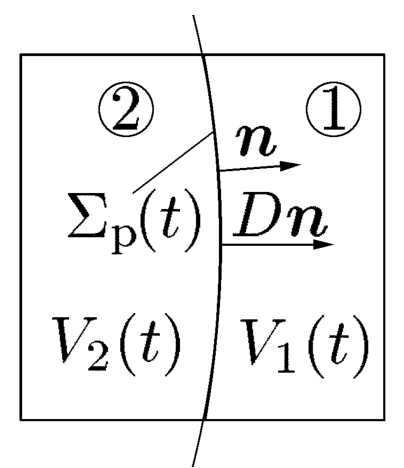
\includegraphics[width=.22\linewidth]{figures/figure-8.png}
\caption{}\label{q3:fig-8}
\end{figure}
где $M$, $\boldsymbol{R}$ и $E$ --- дополнительные поверхностные притоки массы, импульса и энергии на разрыве, которые, вообще говоря, отличны от нуля. Например, при фильтрации воды через границу двух пористых сред с разными пористостями возникает дополнительная поверхностная сила, действующая со стороны скелета на жидкость\setcounter{footnote}{0}\footnote{Природу этой силы легко понять на примере модельного течения через стык двух капилляров с разными диаметрами.}, равная по модулю $|p[m]|$ (при изотермической фильтрации из условия сохранения энергии в этой задаче следует непрерывность давления). Другим примером поверхностной силы может служить возникающая на границе двух жидкостей, находящихся в пористой среде, капиллярная разность давлений, величина которой имеет порядок $R\sim m\sigma/d$, где $\sigma$ --- коэффициент поверхностного натяжения.

Далее мы перечислим некоторые типы граничных условий, встречающихся при решении практических задач.

\topic{Непроницаемая граница}
На границе пористой среды с непроницаемой стенкой или с другой пористой средой, проницаемостью которой можно пренебречь, ставится \textit{условие непротекания} $\boldsymbol{u}\cdot\boldsymbol{n}=0$. Примерами таких границ служат поверхности бетонных оснований гидротехнических сооружений (рис. 1) или границы песка и глины (проницаемость глины на несколько порядков меньше проницаемости песка, поэтому в гидрологических расчетах ее часто рассматривают как непроницаемый материал).

Обратим внимание, что при микроскопическом описании движения жидкости на поверхности пор ставится условие прилипания, т.е. требуется обращение в ноль как нормальной, так и касательной составляющей скорости. При осредненном описании на границе можно поставить условие только на объемный поток
% Источник: Leontiev-2017.pdf; печатная страница: 34; страница файла: 34
жидкости через границу --- он должен быть равен нулю, т.к. стенка непроницаема. Касательная же составляющая скорости фильтрации $\boldsymbol{u}_\tau$ может быть отлична от нуля --- жидкость может мигрировать в пристеночном слое вдоль границы. С математической точки зрения эта разница в граничных условиях связана с тем, что микроскопическое уравнение движения (уравнение Навье--Стокса) содержит вторые производные от скорости по координатам, а макроскопическое уравнение движения (закон Дарси) зависит от скорости алгебраически.

\topic{Граница пористой среды с чистым флюидом}
Во многих задачах встречаются границы пористой среды, насыщенной жидкостью, со внешним объемом той же самой жидкости либо границы пористой среды, в которой фильтруется газ, с тем же газом в свободном состоянии. Такой границей, например, является дно водоема, через которое жидкость (вода) может просачиваться из водоема в грунт (в верхнем бьефе\setcounter{footnote}{0}\footnote{Бьеф (франц. bief) --- часть водоема, реки или канала, примыкающая к водоподпорному сооружению (плотине, шлюзу).} на рис. 1) или, наоборот, через которое грунтовые воды могут проникать в водоем (в нижнем бьефе на рис. 1). Для движения газа такими границами являются, например, внутренняя поверхность скважины, пробуренной в газоносный пласт, через которую газ выходит из пористой среды в ствол скважины, или, скажем, тлеющий кончик сигареты, через который табачный дым выходит в атмосферу (в последнем примере на границе осуществляется поверхностный энергоподвод).

Как правило, на таких границах ставятся условия сохранения массы $[\rho u_n]=0$ и непрерывности давления $[p]=0$ (в задачах изотермического движения несжимаемой жидкости последнее условие следует из закона сохранения энергии).

В водоемах распределение давления с глубиной практически не зависит от наличия течений, поэтому в гидротехнических задачах внешнее давление, как правило, определяется по гидростатическому закону $p=p_{\text{атм}}+\rho gh$, где $h$ --- вертикальное расстояние от рассматриваемой точки на дне до поверхности жидкости. В задачах фильтрации газа обычно можно считать внешние давление и плотность газа заданными постоянными величинами или функциями времени.

% Источник: Leontiev-2017.pdf; печатная страница: 35; страница файла: 35
\topic{Граница раздела фаз внутри пористой среды}
\setcounter{footnote}{0}
Если разные части пористой среды насыщены двумя разными жидкостями или жидкостью и газом, то граница между этими областями является поверхностью разрыва\footnote{Подчеркнем, что здесь не рассматривается многофазная фильтрация (течения смесей, эмульсий, жидкостей с пузырьками газа и т.п. в пористой среде), когда характерные размеры связных областей одной фазы меньше или порядка характерного размера пор.}.

Например, часто при фильтрации грунтовых вод область, в которой поры целиком заполнены водой, и область, в которой поры заполнены воздухом, отделены друг от друга поверхностью, называемой \textit{поверхностью депрессии} или \textit{фреатической поверхностью}\footnote{Депрессия (франц. d\'epression) --- понижение уровня (грунтовых вод); фреатический (греч. $\varphi\rho\varepsilon\alpha\rho$, род. пад. $\varphi\rho\varepsilon\alpha\tau o\varsigma$ --- «колодец», «источник») --- относящийся к грунтовым водам.} (рис.~\ref{q3:fig-9}). В реальности эта граница представляет собой переходную зону некоторой толщины, но при рассмотрении крупномасштабных явлений, встречающихся в гидротехнической практике, эту зону можно моделировать как поверхность. Эта поверхность является \textit{свободной} --- до решения задачи ее форма (кроме тривиального случая горизонтальной поверхности) неизвестна, а в нестационарных задачах поверхность депрессии может менять свою форму с течением времени.

Другим примером границы двух фаз является фронт вытеснения одной жидкостью другой, движущийся внутри пористой среды (при горизонтальном вытеснении такая граница будет устойчивой, если вытесняющая жидкость более вязкая, чем вытесняемая).

\begin{figure}[H]
\centering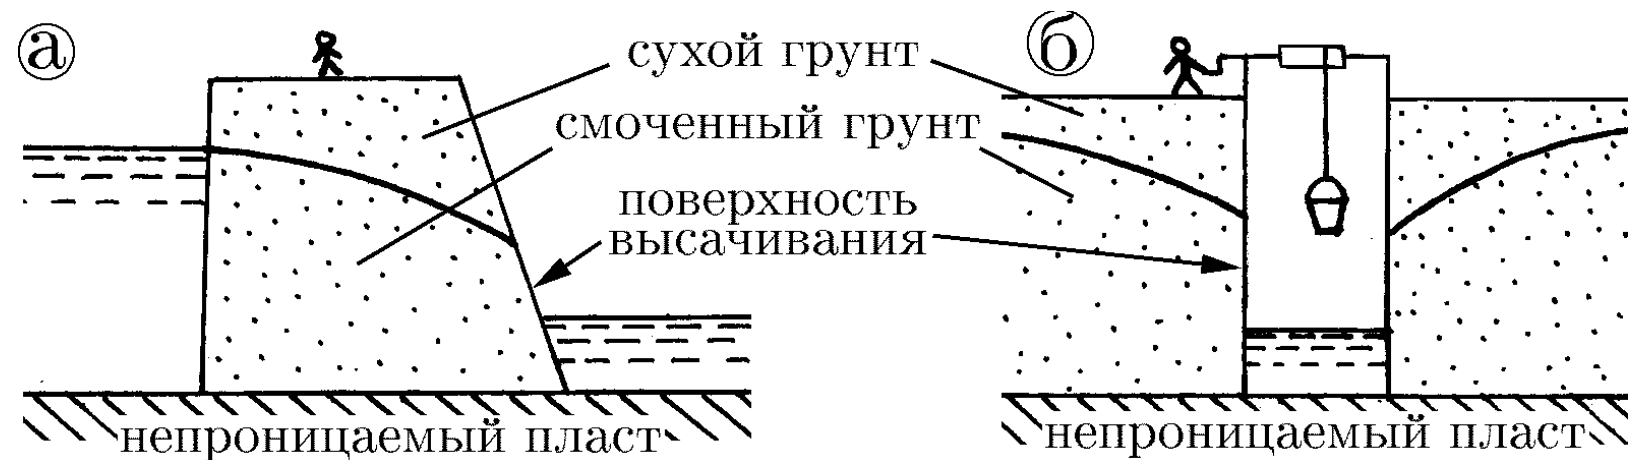
\includegraphics[width=.94\linewidth]{figures/figure-9.png}
\caption{}\label{q3:fig-9}
\end{figure}
При изотермической фильтрации на подвижной границе ставятся обычно общее условие сохранения массы $[\rho(mD-u_n)]=0$ и (в пренебрежении капиллярными силами) условие непрерывности давления $[p]=0$.

% Источник: Leontiev-2017.pdf; печатная страница: 36; страница файла: 36
\topic{Промежуток высачивания}
В ряде гидротехнических задач на части границы пористой среды с атмосферой жидкость может вытекать из пористой среды и, скажем, стекать вдоль границы или испаряться. Такие участки называются \textit{поверхностями высачивания} и встречаются, например, на стенках земляных плотин, через которые фильтруется вода, или на стенках колодцев, вырытых в водонасыщенном грунте (рис.~\ref{q3:fig-9}).

На поверхности высачивания ставятся условия непрерывности давления (в пренебрежении капиллярными эффектами давление жидкости в пористой среде на границе совпадает с атмосферным) и положительности проекции скорости фильтрации на внешнюю нормаль $\boldsymbol{u}\cdot\boldsymbol{n}>0$ (жидкость может только вытекать из пористой среды). Сама же величина скорости фильтрации на границе до решения задачи неизвестна.

\topic{Граница двух пористых сред}
Примерами подобных границ являются поверхности раздела между расположенными рядом природными пластами с разными проницаемостями или, скажем, граница между фильтром и внешней пористой осадочной коркой, откладывающейся на его внешней поверхности при его загрязнении.

\begin{figure}[H]
\centering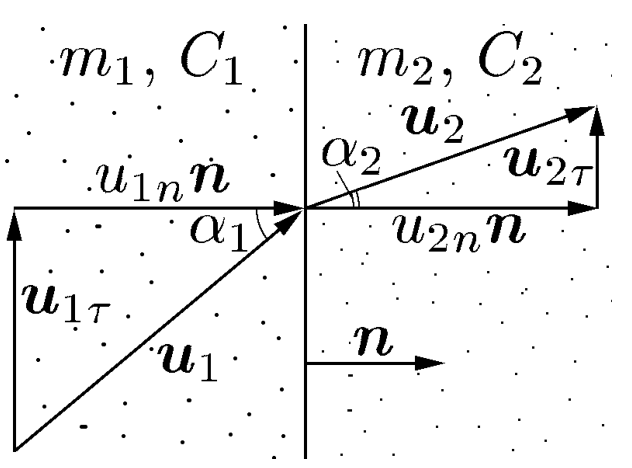
\includegraphics[width=.33\linewidth]{figures/figure-10.png}
\caption{}\label{q3:fig-10}
\end{figure}
При фильтрации несжимаемой жидкости на такой границе ставятся условия непрерывности нормальной компоненты скорости фильтрации $[u_n]=0$ и, как уже говорилось, непрерывности давления $[p]=0$. Отметим, что \textit{касательные} составляющие скорости фильтрации $\boldsymbol{u}_\tau$ по разные стороны от разрыва в общем случае отличаются (рис.~\ref{q3:fig-10}). В самом деле, в силу условия непрерывности давления величина напора $H$ непрерывна на разрыве, поэтому проектирование закона Дарси \eqref{q3:eq-3-6}, записанного по обе стороны поверхности, на касательную плоскость к поверхности дает условие
\[
\frac{|\boldsymbol{u}_{1\tau}|}{C_1}=\frac{|\boldsymbol{u}_{2\tau}|}{C_2},
\]
т.е. касательные составляющие скорости фильтрации относятся как коэффициенты фильтрации. Отсюда, с учетом условия
% Источник: Leontiev-2017.pdf; печатная страница: 37; страница файла: 37
$[u_n]=0$, получается соотношение на углы $\alpha_1$ и $\alpha_2$, которые образуют векторы скорости фильтрации с вектором нормали:
\[
\frac{\operatorname{tg}\alpha_1}{C_1}=\frac{\operatorname{tg}\alpha_2}{C_2}.
\]
Подчеркнем, что в общем случае (например, при фильтрации газа через границу двух сред с разными пористостями, когда внутрипоровые скорости движения частиц газа велики) скачок давления на границе может быть отличен от нуля и должен определяться из дополнительных соотношений\setcounter{footnote}{0}\footnote{Аналогичная ситуация встречается, например, при течении газа в трубе с внезапным расширением или при протекании газа через перфорированные перегородки.}.
% Конец § 6 и главы I. На следующей странице 38 начинается глава II, § 7.
